\documentclass[aspectratio=169]{beamer}

\mode<presentation>
{
    \usetheme{Boadilla}
    \usecolortheme{default}
    \usefonttheme{default}
    \setbeamertemplate{navigation symbols}{}
    \setbeamertemplate{caption}[numbered]
} 

\usepackage[magyar]{babel}
\usepackage[utf8]{inputenc}
\usepackage[T1]{fontenc}
\usepackage{graphicx, tikz}
\usepackage[framemethod=TikZ]{mdframed}

\newcommand\annotatedFigureBoxCustom[8]{
    \draw[#5,ultra thick,rounded corners] (#1) rectangle (#2);
    \node at (#4) [fill=#6,thick,shape=circle,draw=#7,
                   inner sep=2pt,font=\sffamily,text=#8]
                   {\textbf{#3}};
}


% {from}{to}{text}{color}
\newcommand\anbox[4]{\annotatedFigureBoxCustom{#1}{#2}{#3}{#1}{#4}{white}{black}{black}}


\newcommand\antext[5]{
    \draw[#4, fill=#5, ultra thick, rounded corners] (#1) rectangle (#2)
    node[pos=0.5, font=\sffamily, text=black] {\textbf{#3}};
}


\newenvironment{anfig}[1]
{
    \begin{mdframed}[linecolor=blue!65!white, linewidth=2pt, roundcorner=0.75pt,
                     innerrightmargin=0.05pt, innerleftmargin=0.05pt,
                     innertopmargin=0.05pt, innerbottommargin=0.05pt, frametitle={}]
    \begin{tikzpicture}
    \node[anchor=south west,inner sep=0] (image) at (0,0)
    {\includegraphics[width=\textwidth]{#1}};
    \begin{scope}[x={(image.south east)},y={(image.north west)}]
}
{
    \end{scope}
    \end{tikzpicture}
    \end{mdframed}
}

\def\fcol{\color{blue!55!black}}

\newcommand{\fig}[1]{
    \begin{mdframed}[linecolor=blue!65!white, linewidth=1.75pt, roundcorner=0.75pt,
                     innerrightmargin=0pt, innerleftmargin=0pt,
                     innertopmargin=0pt, innerbottommargin=0pt,
                     backgroundcolor=white, frametitle={}, align=center]
        \includegraphics[width=1.0\textwidth]{#1}
    \end{mdframed}
}

\newcommand{\figm}[2]{
    \begin{center}
    \begin{minipage}[c]{#2\textwidth}
    \begin{mdframed}[linecolor=blue!65!white, linewidth=1.75pt, roundcorner=0.75pt,
                     innerrightmargin=0pt, innerleftmargin=0pt,
                     innertopmargin=0pt, innerbottommargin=0pt,
                     backgroundcolor=white, frametitle={}, align=center]
        \includegraphics[width=1.0\textwidth]{#1}
    \end{mdframed}
    \end{minipage}
    \end{center}
}

\newenvironment{minic}[1]
{
    \begin{center}
    \begin{minipage}[c]{#1\textwidth}
}
{
    \end{minipage}
    \end{center}
}


\newenvironment{figp}[4]
{
    \begin{minipage}[c]{#3\textwidth}
    \centering
    #1
    
    #2
    \end{minipage}
    \begin{minipage}[c]{#4\textwidth}
}
{
    \end{minipage}
}


\newcommand{\figc}[2]
{
    \begin{center}
    \begin{mdframed}[linecolor=blue!65!white, linewidth=1.75pt, roundcorner=0.75pt,
                     innerrightmargin=0pt, innerleftmargin=0pt,
                     innertopmargin=0pt, innerbottommargin=0pt,
                     backgroundcolor=white, frametitle={}, align=center]
    
    \includegraphics[width=1.0\textwidth]{#1}
    \end{mdframed}
    #2
    \end{center}
}

\newcommand\sepframe[1] {
    \begin{frame}
        \begin{center}
            \Huge \fcol
            #1
        \end{center}
    \end{frame}
}

\newcommand\bench[2]{
    \begin{minipage}[t]{0.45\textwidth}
        \centering
        \includegraphics[width=\textwidth]{#1}
        \vspace{7.5pt}
        
        LOS deformáció.
    \end{minipage}
    \hspace{5pt}
    \begin{minipage}[t]{0.45\textwidth}
        \centering
        \includegraphics[width=\textwidth]{#2}
        \vspace{7.5pt}
        
        Kálmán-szűréssel integrált GNSS és InSAR mérések.
    \end{minipage}
}

\def\boxcolor{black}
\def\fillcolor{white}
\def\refcolor{orange}


\def\hun{
    \begin{anfig}{hungary_networks_raw.png}
        \anbox{0.27, 0.3}{0.33, 0.4}{A}{\boxcolor}
        \anbox{0.5, 0.4}{0.5525, 0.525}{B}{\boxcolor}
        \anbox{0.465, 0.05}{0.535, 0.15}{C}{\boxcolor}
    \end{anfig}
}

\def\erdely{
    \begin{anfig}{transylvania_networks_raw.png}
        \anbox{0.4075, 0.55}{0.4875, 0.67}{A}{\boxcolor}
        \anbox{0.55, 0.37}{0.63, 0.49}{B}{\boxcolor}
        \anbox{0.75, 0.08}{0.9, 0.4}{C}{\boxcolor}
    \end{anfig}
}

\def\dszekcso{
    \begin{anfig}{dszekcso_network_raw.png}
        \antext{0.05, 0.57}{0.25, 0.64}{IB1}{\refcolor}{\fillcolor}
        \antext{0.3, 0.67}{0.5, 0.74}{IB2}{\boxcolor}{\fillcolor}
        \antext{0.225, 0.47}{0.425, 0.54}{IB3}{\boxcolor}{\fillcolor}
        \antext{0.32, 0.25}{0.52, 0.32}{IB4}{\boxcolor}{\fillcolor}
    \end{anfig}
}

\def\kulcs{
    \begin{anfig}{kulcs_network_raw.png}
        \antext{0.125, 0.875}{0.225, 0.975}{A1}{\boxcolor}{\fillcolor}
        \antext{0.51, 0.45}{0.61, 0.55}{A2}{\boxcolor}{\fillcolor}
        \antext{0.825, 0.17}{0.925, 0.27}{A3}{\boxcolor}{\fillcolor}
        \antext{0.79, 0.04}{0.89, 0.14}{A4}{\boxcolor}{\fillcolor}
        \antext{0.46, 0.17}{0.56, 0.27}{AR}{\refcolor}{\fillcolor}
        \antext{0.475, 0.7}{0.625, 0.8}{Duna}{\boxcolor}{\fillcolor}
    \end{anfig}
}

\def\fonyod{
    \begin{anfig}{fonyod_network_raw.png}
        \antext{0.25, 0.78}{0.45, 0.86}{Balaton}{\boxcolor}{\fillcolor}
        \antext{0.725, 0.77}{0.825, 0.87}{KV}{\boxcolor}{\fillcolor}
        \antext{0.725, 0.16}{0.825, 0.26}{PH}{\refcolor}{\fillcolor}
        \antext{0.29, 0.0575}{0.39, 0.1575}{RE}{\boxcolor}{\fillcolor}
    \end{anfig}
}


\def\csomad{
    \begin{anfig}{ciomadul_network_raw.png}
        \antext{0.3, 0.29}{0.42, 0.375}{C1}{\boxcolor}{\fillcolor}
        \antext{0.21, 0.1}{0.33, 0.18}{C2}{\refcolor}{\fillcolor}
        \antext{0.665, 0.2}{0.775, 0.28}{C3}{\boxcolor}{\fillcolor}
        \antext{0.49, 0.565}{0.6, 0.645}{C4}{\boxcolor}{\fillcolor}
        \antext{0.64, 0.82}{0.76, 0.9}{C5}{\refcolor}{\fillcolor}
    \end{anfig}
}



\graphicspath{{../../images/}}


\title[XI. Geomatika Szeminárium, Sopron 2018]{Lassú felszíni deformációs folyamatok monitorozása sarokreflektorok és Sentinel-1 adatok felhasználásával magyarországi teszt területeken}
\author[Bozsó et al.]{Bozsó István, Szűcs Eszter, Bányai László, Wesztergom Viktor}
\institute[MTA CSFK GGI]{MTA CSFK Geodéziai és Geofizikai Intézet}
\date{2018.11.08.}


\begin{document}

\begin{frame}
    \titlepage
    \begin{center}
        \begin{minipage}[c]{0.25\textwidth}
            
\includegraphics[width=0.75\textwidth]{ggi_logo.png}
        \end{minipage}
        \hspace{30pt}
        \begin{minipage}[c]{0.25\textwidth}
            
\includegraphics[width=0.75\textwidth]{esa_logo.eps}
        \end{minipage}
    \end{center}
\end{frame}

\begin{frame}{Áttekintés}
    \tableofcontents
\end{frame}

\section{A reflektorok tervezése}

\begin{frame}{A reflektorok tervezése}
    \textbf{ESA-PECS pályázat} keretében: reflektorok tervezése, telepítése, mérések feldolgozása.
    \vspace{10pt}
    
    Szempontok:
    \begin{itemize}
        \item analóg, analitikus és numerikus számítások - BME Szélessávú Hírközlés és Villamosságtan Tanszék
        \item Sentinel-1 radar hullámhossz és pályaparaméterek,
        \item mechanikai kompaktság és stabilitás.
    \end{itemize}
    \begin{center}
        \resizebox{0.1\textwidth}{30pt}{$\Downarrow$}
        \vspace{10pt}
        
        optimális reflektor geometria
    \end{center}    
\end{frame}


\subsection{Alapfogalmak}

\begin{frame}{Alapfogalmak}
    A hatásos radarszórási keresztmetszet (Radar cross-section, RCS), visszaverő képesség:
    
    \begin{equation*}
        \sigma = 4 \pi \lim_{R \to \infty} R^2 \frac{ \abs{\subt{E}{szórt}}^2 }{ \abs{\subt{E}{beeső}}^2 },
    \end{equation*}
    
    ahol
    
    \begin{itemize}
        \item $R$ meggfigyelési pont távolsága a céltárgytól,
        \item $\subt{E}{szórt}$ szórt elektromágnese térerősség,
        \item $\subt{E}{beeső}$ céltárgyra beérkező elektromágnese térerősség.
    \end{itemize}
    
    Mértékegysége: $\dbm$
    
\end{frame}


\subsection{Reflektor típusok}

\begin{frame}{Reflektor típusok}
    \begin{center}
        \begin{minipage}[c]{0.75\textwidth}
            \begin{minipage}[t]{0.41\textwidth}
                \centering
                \reflector{reflector_triangle.png}{a}
            \end{minipage}
            \hspace{2pt}
            \begin{minipage}[t]{0.37\textwidth}
                \centering
                \reflector{reflector_pentagonal.png}{b}
            \end{minipage}
            \vspace{5pt}
            
            \begin{minipage}[t]{0.44\textwidth}
                \centering
                \reflector{reflector_circular.png}{c}
            \end{minipage}
            \hspace{2pt}
            \begin{minipage}[t]{0.4\textwidth}
                \centering
                \reflector{reflector_rectangular.png}{d}
            \end{minipage}        
        \end{minipage}
        \begin{minipage}[c]{0.225\textwidth}
            \begin{itemize}
                \item \textbf{a}: Háromszög
                \item \textbf{b}: Pentagonális
                \item \textbf{c}: Negyedkör
                \item \textbf{d}: Négyzet
            \end{itemize}
        \end{minipage}
    \end{center}
\end{frame}


\begin{frame}
    \begin{minipage}[t]{0.475\textwidth}
        \centering
        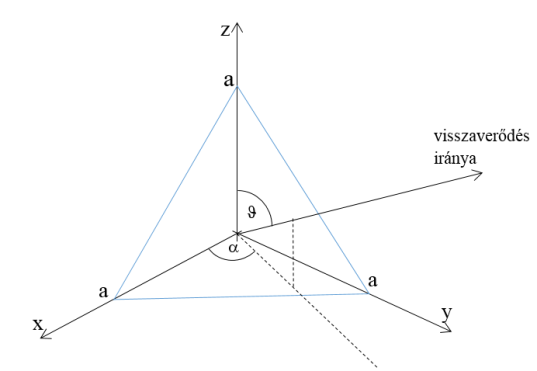
\includegraphics[width=\textwidth]{reflector_angles.png}
        
        A beesési irányt jellemző két szög. $\alpha$: azimuth, $\vartheta$: beesési szög.
    \end{minipage}
    \begin{minipage}[t]{0.475\textwidth}
        \centering
        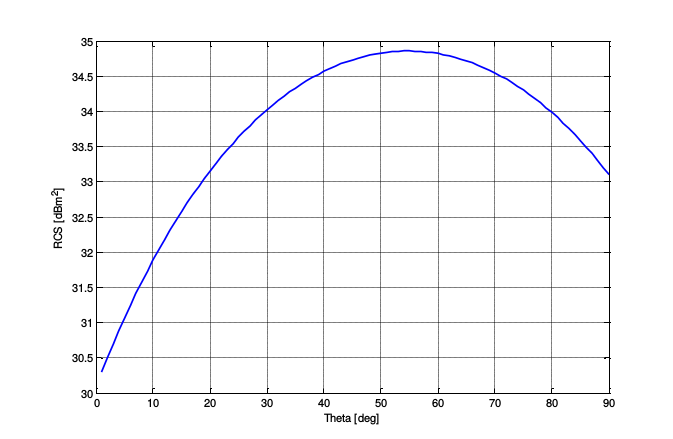
\includegraphics[width=\textwidth]{trihedral_theo.png}
        
        Elméleti számítások alapján felrajzolt RCS a beesési szög függvényében háromszög reflektorra. $a = \SI{1}{\meter} $, $f = \SI{5.405}{\giga\hertz}$, $\text{azimuth} = \SI{45}{\degree}$. Maximum RCS $\SI{55}{\degree}$ beesési szögnél.
    \end{minipage}
\end{frame}


\subsection{Numerikus modellezés eredményei}

\sepframe{Numerikus modellezés eredményei}

\begin{frame}{Különböző reflektortípusok RCS karakterisztikái}
    \begin{minipage}[c]{0.55\textwidth}
        \centering
        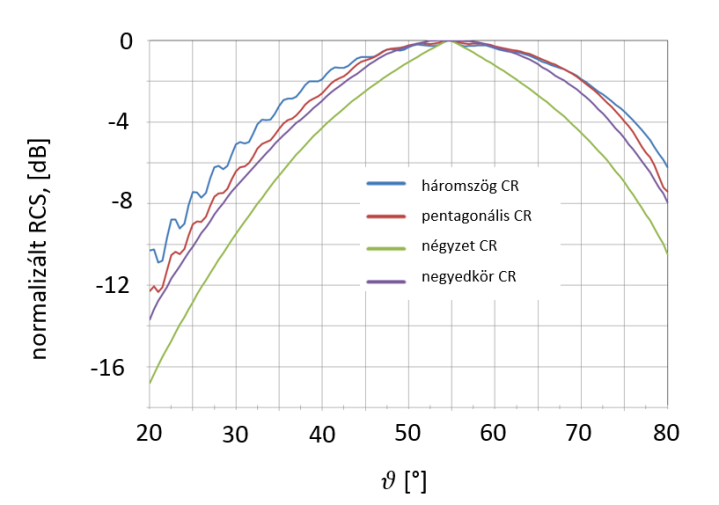
\includegraphics[width=\textwidth]{reflectors_compare_elevation.png}
        
        Különböző reflektorok normalizált RCS görbéi a beesési szög függvényében. $a = \SI{1}{\meter} $, $f = \SI{5.405}{\giga\hertz}$, $\text{azimuth} = \SI{45}{\degree}$
    \end{minipage}
    \hspace{5pt}
    \begin{minipage}[c]{0.325\textwidth}
        \begin{table}
            \centering
            \begin{tabular}{m{75pt} c} \toprule
                Típus & Szögátmérő (3 $\db$) \\ \midrule
                Háromszög & $\SI{38.2}{\degree}$ \\ \hline
                Pentagonális (Csonkolás: $\SI{0.25}{\meter}$)& $\SI{34.5}{\degree}$ \\ \hline
                Négyzet & $\SI{22.5}{\degree}$ \\ \hline
                Negyedkör & $\SI{31.3}{\degree}$ 
            \end{tabular}
        \end{table}
    \end{minipage}
\end{frame}


\begin{frame}{Különböző reflektortípusok RCS karakterisztikái}
    \begin{minipage}[c]{0.55\textwidth}
        \centering
        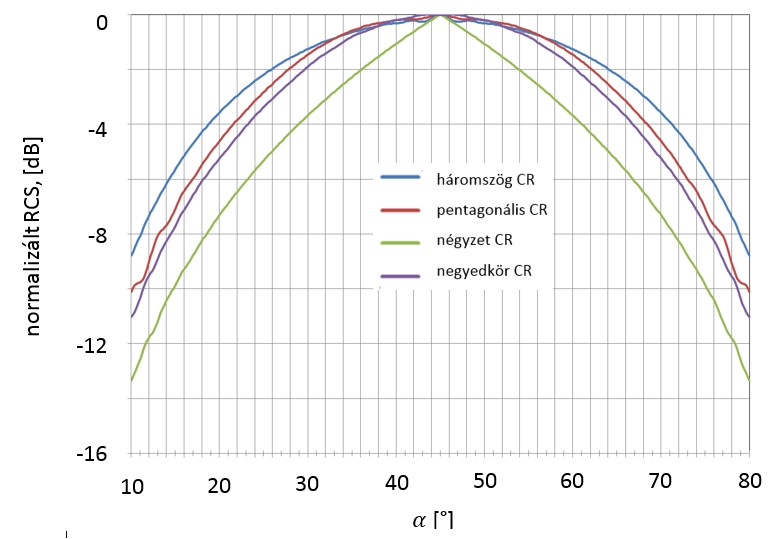
\includegraphics[width=\textwidth]{reflectors_compare_azimuth.png}
        
        Különböző reflektorok normalizált RCS görbéi az azimuth függvényében. $a = \SI{1}{\meter} $, $f = \SI{5.405}{\giga\hertz}$, $\text{beesési szög} = \SI{54.74}{\degree}$
    \end{minipage}
    \hspace{5pt}
    \begin{minipage}[c]{0.325\textwidth}
        \begin{table}
            \centering
            \begin{tabular}{m{75pt} c} \toprule
                Típus & Szögátmérő (3 $\db$) \\ \midrule
                Háromszög & $\SI{46.3}{\degree}$ \\ \hline
                Pentagonális (Csonkolás: $\SI{0.25}{\meter}$)& $\SI{41.1}{\degree}$ \\ \hline
                Négyzet & $\SI{25.3}{\degree}$ \\ \hline
                Negyedkör & $\SI{37.6}{\degree}$
            \end{tabular}
        \end{table}
    \end{minipage}
\end{frame}

\subsection{Optimális reflektor geometria}

\begin{frame}{Optimális reflektor geometria}
    Választás: Pentagonális reflektor
    
    \begin{itemize}
        \item Megfelelően nagy RCS-t szolgáltat.
        \item Mechanikailag stabilabb.
        \item További vizsgálatok alapján az optimális csonkolás aránya: $\frac{\subt{a}{csonkolt}}{a}: 0.4$.
    \end{itemize}
\end{frame}


\begin{frame}{Analóg mérések - reflektor asszimmetria}
    \begin{minipage}[c]{0.65\textwidth}
        \centering
        \inc{reflector_asymmetry.png}
        
        Szembenálló modell reflektorok RCS görbéi az azimuth függvényében.
    \end{minipage}
    \begin{minipage}[c]{0.3\textwidth}
        \centering
        Kísérleti elrendezés.
        \vspace{10pt}
        
        \begin{minipage}[c]{\textwidth}
            \fig{reflector_model_f2f.png}
        \end{minipage}
        \vspace{10pt}
        
        \begin{minipage}[c]{\textwidth}
            \fig{reflector_analogue.png}
        \end{minipage}
    \end{minipage}
\end{frame}

\begin{frame}{Mért intenzitásértékek - Dunaszekcső}
    \begin{minipage}[t]{0.45\textwidth}
        \centering
        \inc{dszekcso_intensity_range.png}
    \end{minipage}
    \hspace{10pt}
    \begin{minipage}[t]{0.45\textwidth}
        \centering
        \inc{dszekcso_intensity_azimuth.png}
    \end{minipage}
    
    \begin{center}
        A dunaszekcsői hálózat környezetében mért relatív intenzitásértékek a távolság függvényében két metszet (range, azimut) esetén.
    \end{center}
\end{frame}


\section{A reflektor hálózatok első eredményei}

\sepframe{Magyarországi reflektor hálózatok és az első eredmények}

\subsection{Dunaszekcsői hálózat}

\begin{frame}{Magyarországi reflektor hálózatok}
    \centering
    \begin{minipage}[c]{0.7\textwidth}
        \hun
        \begin{center}
            \textbf{A}: Fonyód,
            \textbf{B}: Kulcs,
            \textbf{C}: Dunaszekcső
        \end{center}
    \end{minipage}
\end{frame}


\begin{frame}{Magyarországi reflektor hálózatok}
    \begin{minipage}[c]{0.365\textwidth}
        \centering
        \dszekcso

        Dunaszekcsői hálózat
    \end{minipage}
    \hspace{10pt}
    \begin{minipage}[c]{0.58\textwidth}
        \centering
        \kulcs

        Kulcsi hálózat
    \end{minipage}
\end{frame}


% ***************
% * Dunaszekcső *
% ***************


\begin{frame}{Dunaszekcsői hálózat IB2-IB1}
    \bench{IB2-IB1_los.eps}{IB2-IB1_kalman.eps}
\end{frame}

\begin{frame}{Dunaszekcsői hálózat IB3-IB1}
    \bench{IB3-IB1_los.eps}{IB3-IB1_kalman.eps}
\end{frame}

\begin{frame}{Dunaszekcsői hálózat IB4-IB1}
    \bench{IB4-IB1_los.eps}{IB4-IB1_kalman.eps}
\end{frame}

\subsection{Kulcsi hálózat}

\begin{frame}{Magyarországi reflektor hálózatok}
    \begin{minipage}[c]{0.365\textwidth}
        \centering
        \dszekcso

        Dunaszekcsői hálózat
    \end{minipage}
    \hspace{10pt}
    \begin{minipage}[c]{0.58\textwidth}
        \centering
        \kulcs

        Kulcsi hálózat
    \end{minipage}
\end{frame}


% *********
% * Kulcs *
% *********


\begin{frame}{Kulcsi hálózat A1-AR}
    \bench{A1-AR_los.eps}{A1-AR_kalman.eps}
\end{frame}


\begin{frame}{Kulcsi hálózat A3-AR}
    \bench{A3-AR_los.eps}{A3-AR_kalman.eps}
\end{frame}

\subsection{Fonyódi hálózat}

\begin{frame}{Magyarországi reflektor hálózatok}
    \begin{minipage}[c]{0.6\textwidth}
        \centering
        \fonyod

        Fonyódi hálózat
    \end{minipage}
    \hspace{5pt}
    \begin{minipage}[c]{0.3\textwidth}
            \textbf{PH}: Polgármesteri hivatal\\
            \textbf{RE}: Ripka emlékmű\\
            \textbf{KV}: Kripta-villa
    \end{minipage}
\end{frame}


% **********
% * Fonyód *
% **********

\begin{frame}{Fonyód network KV-PH}
    \bench{KV-PH_los.eps}{KV-PH_kalman.eps}
\end{frame}

\begin{frame}{Fonyód network RE-PH}
    \bench{RE-PH_los.eps}{RE-PH_kalman.eps}
\end{frame}

\section{Összefoglalás}

\begin{frame}{Összefoglalás}
    \begin{itemize}
        \item A reflektorok megfelelő mértékű visszavert intenzitás értékeket szolgáltatnak, kiemelkednek környezetükből.
        \item A GNSS és az InSAR reflektor mérések integrálásával 3D-s elmozdulás értékeket kaphatunk kiváló időbeli felbontással (6 naponta).
    \end{itemize}
\end{frame}

\begin{frame}
    \begin{center}
        \Huge \color{blue!55!black}
        Köszönöm a figyelmet!
    \end{center}
    \vspace{35pt}
    {\large
    Acknowledgement: Contains modified Copernicus Sentinel-1 data [2018]
    }
\end{frame}


\backupbegin

\section*{Telepített és tervezett erdélyi hálózatok}

\begin{frame}{Erdélyi reflektor hálózatok}
    \centering
    \begin{minipage}[c]{0.65\textwidth}
        \erdely
        \begin{center}
            \textbf{A}: Parajdi hálózat, 
            \textbf{B}: Csomádi hálózat, 
            \textbf{C}: Vrancea-zóna
        \end{center}
    \end{minipage}
\end{frame}


\begin{frame}{Parajdi hálózat}
    \begin{minipage}[c]{0.7\textwidth}
        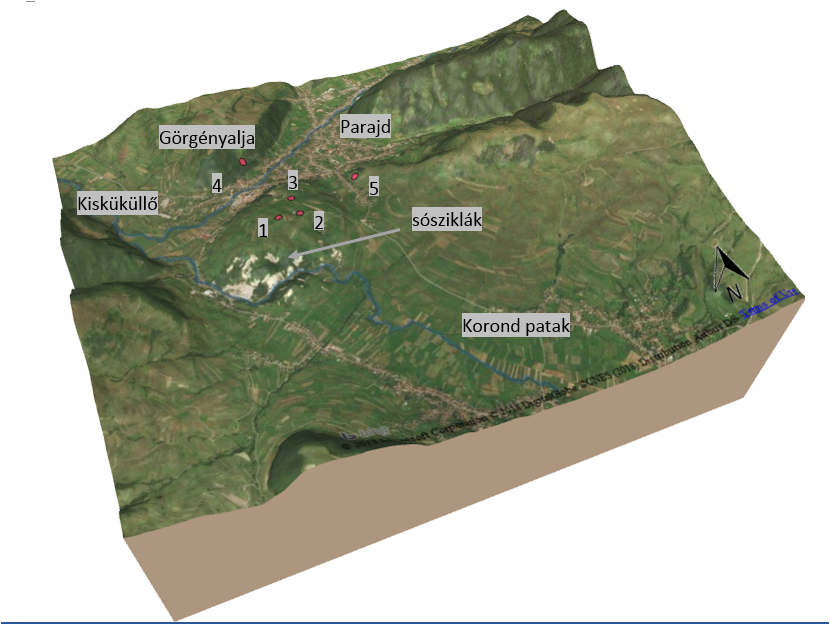
\includegraphics[width=\textwidth]{parajd_3D.png}
    \end{minipage}
    \hspace{5pt}
    \begin{minipage}[c]{0.225\textwidth}
        \begin{itemize}
            \item Közép-Európa legnagyobb sódiapírja $\rightarrow$ sótektonika
            \item vertikális mozgások?
        \end{itemize}
    \end{minipage}
\end{frame}


\begin{frame}{Csomádi hálózat}
    \begin{minipage}[c]{0.475\textwidth}
        \centering
        \csomad
    \end{minipage}
    \hspace{5pt}
    \begin{minipage}[c]{0.45\textwidth}
        \begin{itemize}
            \item magnetotellurikus mérések $\rightarrow$ potenciálisan aktív magmatározó
            \item lehetséges mozgások a Csomád-vulkán környezetében
        \end{itemize}
    \end{minipage}
\end{frame}

\backupend

\end{document}
